\documentclass[10pt,twocolumn]{article}
\usepackage[margin=0.6in]{geometry}
\usepackage{graphicx}
\usepackage{booktabs}
\usepackage{amsmath}
\usepackage{amssymb}
\usepackage[dvipsnames]{xcolor}
\usepackage{titlesec}
\usepackage[font=footnotesize,labelfont=bf]{caption}
\usepackage{lmodern}
\usepackage{microtype}
\usepackage{stfloats}
\usepackage{enumitem}

\definecolor{ink}{HTML}{0A1638}
\definecolor{navy}{HTML}{2E5CA6}
\definecolor{amber}{HTML}{D97706}
\titleformat*{\section}{\large\bfseries\color{ink}}
\titleformat*{\subsection}{\normalsize\bfseries\color{ink}}
\setlength{\parskip}{2pt}
\renewcommand{\topfraction}{0.95}
\renewcommand{\dbltopfraction}{0.95}
\renewcommand{\textfraction}{0.05}
\renewcommand{\dblfloatpagefraction}{0.90}
\setcounter{dbltopnumber}{3}

\title{\vspace{-1.2em}\textbf{Epistemic collapse in multi-agent systems}}
\author{Helivan \quad Johns Hopkins}
\date{September 2026 --- working summary}

\begin{document}
\maketitle

\section*{Motivation}
In the simulation framework of \emph{Control Charts for Multi-agent
Systems} (arXiv:2605.11135), $N$ LLM agents each hold a vector memory,
answer questions from a shared pool by retrieving from that memory,
exchange answers with peers, and are instructed to say ``I don't know''
(IDK) when retrieval provides no grounding. That paper studied an
\emph{exogenous} failure --- adversarial injection --- and asked whether
statistical monitoring detects it. This project studies the
\emph{endogenous} failure: the regime in which an agent, or every agent,
can answer with nothing but IDK. We call this \textbf{epistemic
collapse}, and we want to know when it happens, whether it is a sharp
threshold or a graded frontier, how fast it arrives, which factors drive
it, and whether the two natural levels --- \emph{agent-level} (a given
agent cannot answer) and \emph{system-level} (no agent can answer) ---
move together or apart. Sitting behind all of this is a trade-off the
static framework cannot express: in a changing world, an agent that
retains evidence too long is \emph{wrong}, and one that discards it fast
enough to be right may fall below the threshold at which the collective
can know anything at all.

\section*{Framework}
\textbf{Model.} We work with a deliberately small model (toy simulator
v2) that keeps the paper's ask/answer/IDK mechanics but adds the
variables the question needs. $N$ agents face $M$ questions; question $q$
changes each step with probability $\lambda_q$ (log-normal across
questions, mean $\bar\lambda$, dispersion $\sigma_\lambda$; static
questions are the $\lambda_q\to0$ limit). Every stored answer carries two
timestamps: $t_{\mathrm{obs}}$, when it was observed from the
environment --- \emph{provenance travels unchanged through exchange} ---
and $t_{\mathrm{recv}}$, when this agent received its copy; on receiving
a duplicate, the newer $t_{\mathrm{obs}}$ wins. Each agent spends a
budget of $B$ actions per step: a fraction $\alpha$ observing the
environment (question drawn from $\pi_{\mathrm{env}}$, observation exact
and freshly stamped) and the rest asking peers (question drawn by policy
$\sigma$ weighted by demand $\pi_{\mathrm{ask}}$, peer drawn on contact
graph $G$). An agent \emph{answers} $q$ only if its estimated probability
of still being right, $e^{-\lambda_q(t - t_{\mathrm{obs}})}$, is at least
a caution level $c$ --- so evidence expires at age
$\theta_q = \ln(1/c)/\lambda_q$ --- and only if it received its copy
within a memory lifetime $\tau$.

\textbf{Metrics.} Agent-level collapse probability
$P(\mathrm{IDK}) = 1 - \overline{\mathrm{knows}}$ over (agent, question)
pairs; system-level collapse $P(\mathrm{dead})$ = fraction of questions
no agent can answer; the answers actually given split into correct
vs.\ stale. All are means over the last 200 of 800 steps, 10 seeds.

\textbf{Mean-field picture.} Per question, knowledge is a
susceptible--infected--susceptible contagion: a copy is born when an ask
reaches a holder, and dies when it expires. With bandwidth
$m = (1-\alpha)B$ this gives a reproduction number
$R_0 \approx m\tau/M$, $N$-invariant to first order. Three timescales
organise everything: memory $\tau$, the per-question observation interval
$M/(\alpha B N)$, and evidence validity $\theta_q$. If $\tau = \infty$,
communication cannot affect system-level survival at all --- a lineage
dies $\theta_q$ after observation no matter how much it circulates ---
and only spreads evidence farther (agent level). Communication becomes
load-bearing at the system level exactly when
$\tau < M/(\alpha B N) < \theta_q$: the observer forgets before anyone
re-observes and before the evidence goes stale, so a lineage survives
only by circulating --- the SIS threshold confined to the validity
window. A healthy system needs all three conditions at once:
$m\tau/M \gtrsim 1$ (spread), $\theta_q$ large enough relative to
re-observation (someone is watching in time), and caution matched to
speed (don't be stale). The candidate headline result is that the
feasibility window closes entirely when the environment is fast enough
relative to bandwidth --- the epistemic analogue of the control-chart
paper's learning--security trade-off.

\section*{Experimental setup}
Two standalone numpy simulators, both implementing the repo's
asking/answering rules. \textbf{v1} (receipt-clock expiry $\tau_{mem}$,
independent ask rate $K$ and observation rate $\varepsilon$, no caution)
exists to test the SIS prediction cleanly. \textbf{v2} is the model
above. The published simulator itself has none of these levers ---
memory never expires (a control run confirmed it cannot produce
system-level death at any pool size: without a death term, knowledge
only accumulates), so the toy models carry the design until the repo is
extended. The v2 design is a factor-structured sweep: variables sort
into four factors --- \emph{agent}, \emph{communication},
\emph{environment}, \emph{observation} (the environment$\to$agent
interface) --- and each factor contributes one panel varying its
intrinsic lever with two secondary variables (lightness / line-style),
all other factors held at a common baseline chosen so the three clocks
are ordered $\tau < M/(\alpha BN) < \theta$: $N{=}20$, $M{=}50$,
$B{=}5$, $\alpha{=}0.01$ (99 asks per observation), $\tau{=}20$,
$c{=}0.5$, $\bar\lambda{=}0.003$ ($\theta\approx231$, $R_0\approx2$),
flat $\pi_{\mathrm{env}}$ and $\pi_{\mathrm{ask}}$, full mesh. At
baseline the system is healthy: $P(\mathrm{IDK})=0.14$,
$P(\mathrm{dead})=0.02$. The full grid is 1{,}380 runs
($\approx$75\,s on 30 cores), so iteration is effectively free.

\begin{figure*}[t]
  \vspace{-6pt}\centering
  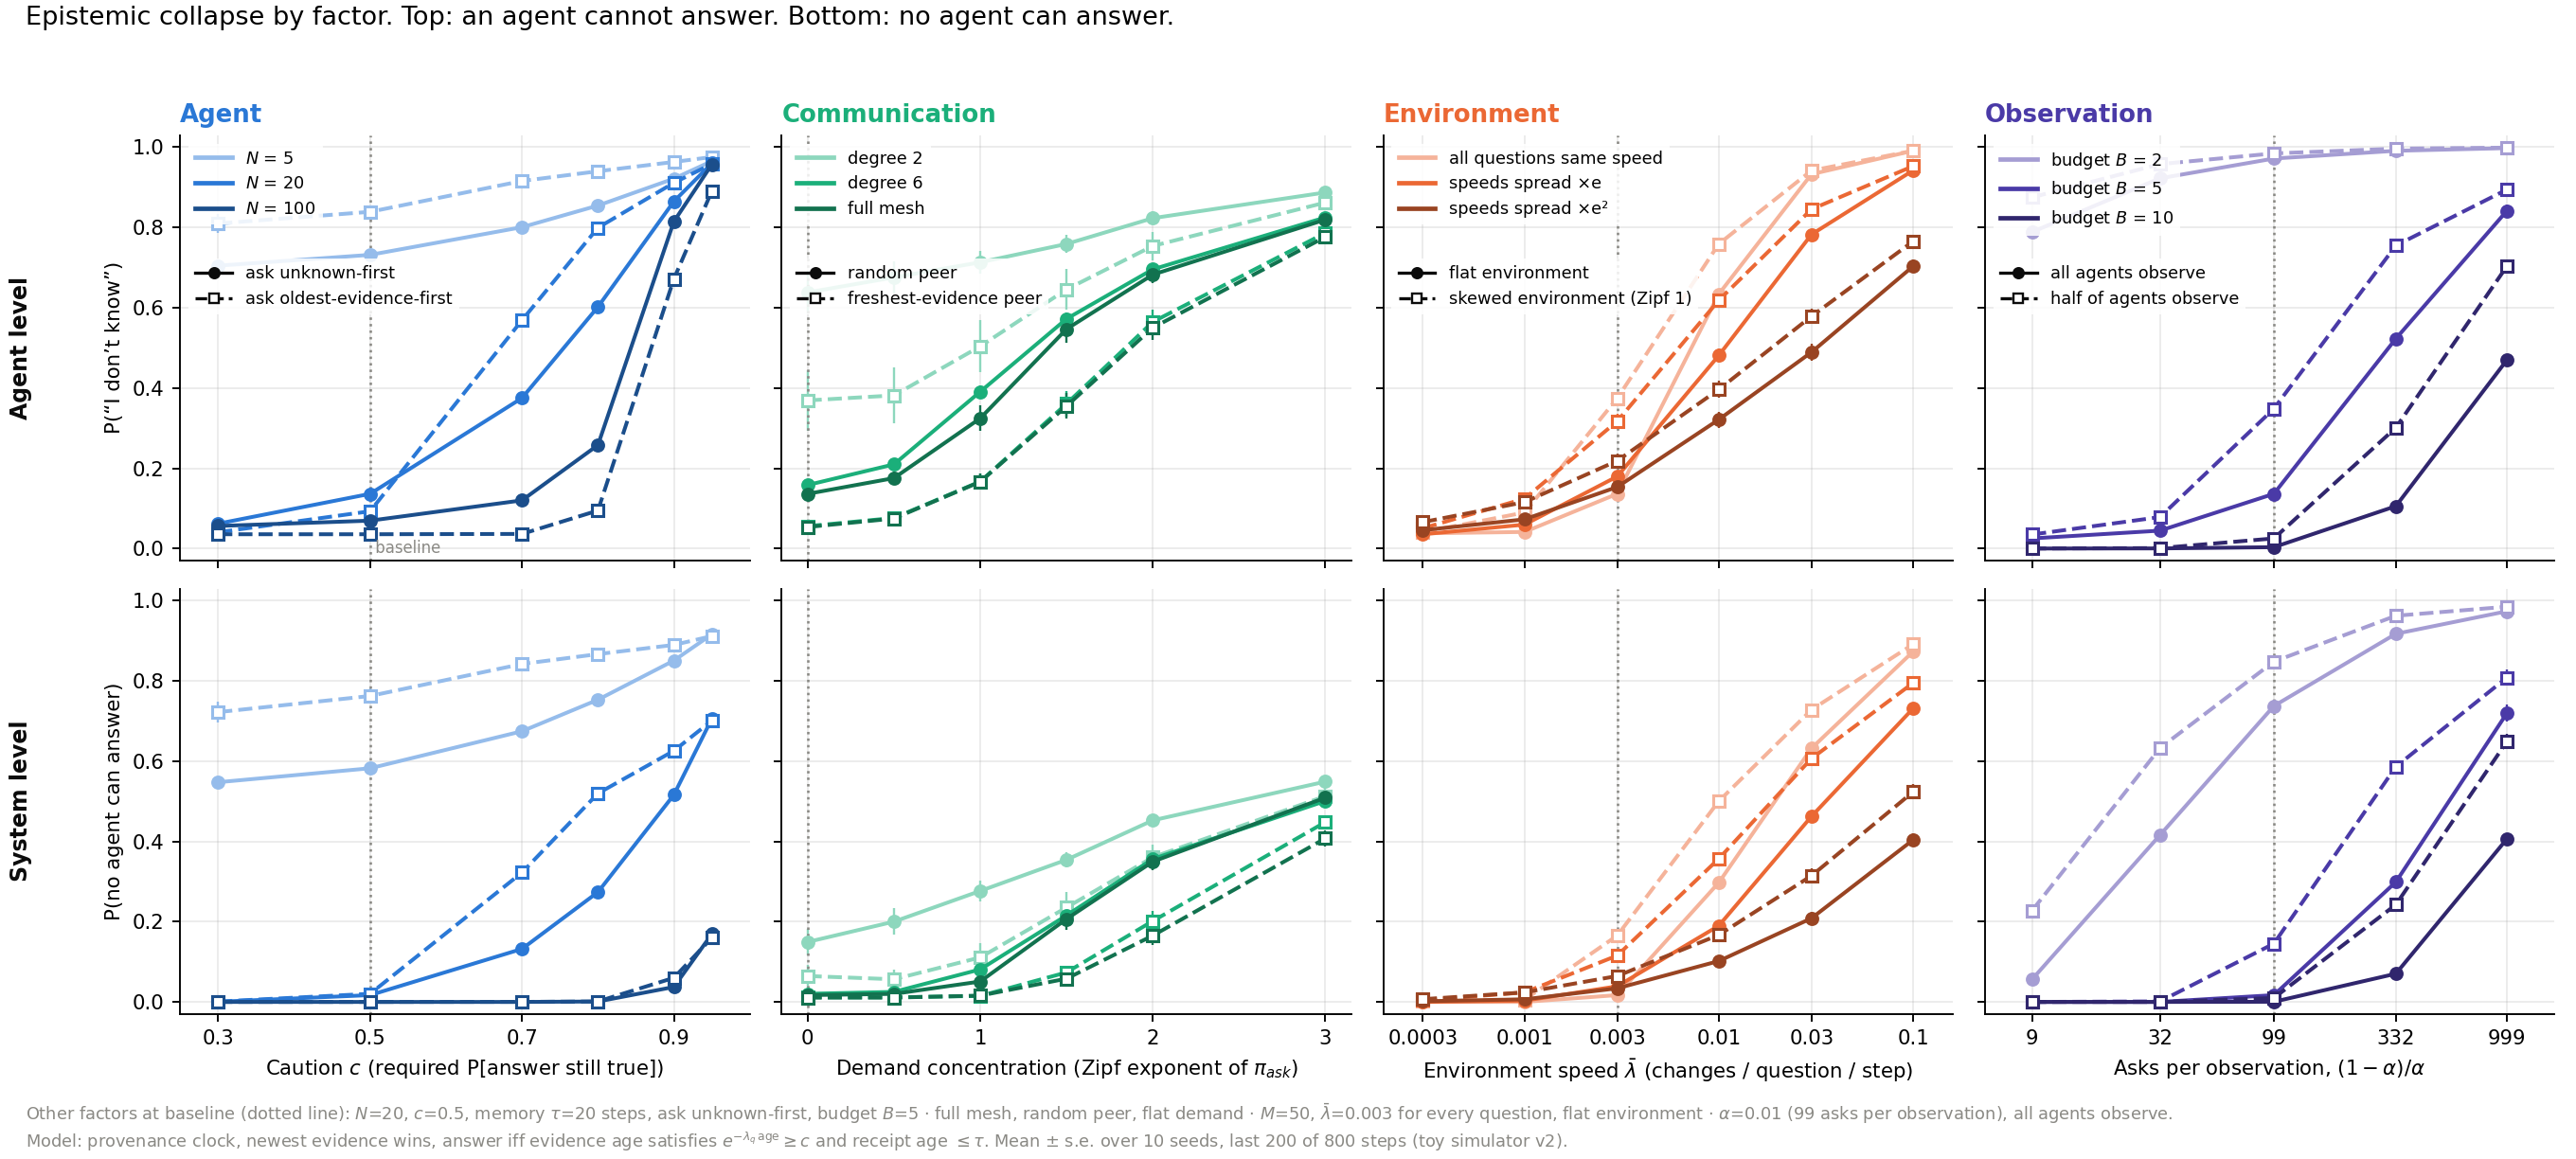
\includegraphics[width=\textwidth]{../figure1_collapse_by_factor.png}
  \caption{One intrinsic lever per factor carries the system from
  healthy to collapsed at both levels. Top row: agent-level
  $P(\mathrm{IDK})$; bottom row: system-level $P(\text{no agent can
  answer})$; dotted vertical = the common baseline. Hue = factor;
  lightness = the factor's second variable; solid-filled
  vs.\ dashed-hollow = its third.}
  \label{fig:factors}
\end{figure*}

\section*{Results}
\textbf{v1: collapse is an SIS threshold.} With expiry on the receipt
clock, the fraction of questions alive collapses as a function of
$R_0 = K\tau_{mem}/M$ alone, with the transition at
$R_0\approx1.25$--$1.5$ for $N\in\{5,20,100\}$ (slightly above the
mean-field 1, from duplicate asks and founder extinctions); time to
system collapse diverges approaching the threshold, and $N$ sets how
long extinction takes, not whether it happens. An environment channel
decouples the two levels: at $R_0=0.5$, observation at
$\varepsilon\ge0.3$ keeps $\sim$95\% of questions alive somewhere while
every agent remains $>$90\% IDK --- and the linearised SIS source term
predicts the agent-level numbers to within a point (predicted 0.94, 0.80
at $\varepsilon=0.3,1$; observed 0.94, 0.81). Skewing which questions
the world reveals is the environment's real lever (IDK
$0.03\to0.57$ at $M{=}100$ as normalised entropy falls to 0.2), and it
matters precisely when the system leans on observation to stay alive.
Skewing \emph{demand} instead kills the tail invisibly: uniform-weighted
IDK reaches 0.56 at Zipf $s{=}2$ while demand-weighted IDK sits at
0.01--0.04 --- a probe that samples questions the way agents ask them
cannot see the collapse. Collapse under rarity is a frontier moving
inward, not a single threshold.

\textbf{v2: every factor owns a lever to collapse
(Fig.~\ref{fig:factors}).} \emph{Agent --- caution.} IDK rises from 0.06
at $c=0.3$ to 0.96 at $c=0.95$ (system death $0\to0.71$); small
populations start collapsed ($N{=}5$: IDK 0.71 at $c=0.3$, because
observations per question scale with $\alpha BN$). Asking
oldest-evidence-first lowers agent-level IDK but \emph{raises}
system-level death (0.32 vs.\ 0.13 at $c=0.7$): re-verifying what you
hold spends asks that would have carried rare lineages. Raising caution
trades stale for IDK (stale $0.19\to0.00$ as IDK $0.06\to0.96$); at
baseline speed the not-correct optimum sits at or below $c=0.3$.
\emph{Communication --- demand concentration.} Zipf demand takes IDK
$0.14\to0.82$ and death $0.02\to0.51$ ($s:0\to3$) on the mesh; a
degree-2 graph starts at IDK 0.64. Freshest-evidence peer selection
roughly halves agent-level IDK at every $s$ but delivers much less at
the system level (death 0.41 vs.\ 0.51 at $s{=}3$): it redistributes
evidence, it cannot create it. \emph{Environment --- speed.} Death goes
$0.02\to0.87$ across $\bar\lambda = 0.003\to0.1$; through caution, speed
is one of the steepest levers (in v1, with no caution, it had no effect
on IDK at all). Spreading speeds across questions protects the mean
(death 0.21 vs.\ 0.63 at $\bar\lambda=0.03$, dispersion $\times e^2$):
collapse concentrates on the volatile minority. \emph{Observation ---
asks per observation.} From 99 to 999 asks per observation, death goes
$0.02\to0.72$ at $B{=}5$; a budget of 10 tolerates roughly $3\times$ the
ratio (death 0.41 at 999). The recurring structural finding is the
agent/system split: policies and topology move agent-level ignorance
freely, but only the observation channel creates evidence, and only
memory--bandwidth--pool-size ($R_0$) decides whether created evidence
survives.

\section*{Remaining tasks}
\begin{enumerate}[leftmargin=1.4em,itemsep=1pt,topsep=1pt]
  \item Re-scope the planned experiment series to v2: the
  $(m,\tau,M)$ phase diagram inside the validity window, speed
  $\times$ caution (the closing feasibility window --- headline), and
  topology/heterogeneity (who collapses first).
  \item An analytic treatment of the feasibility window
  $\tau \in (M/m,\;\theta)$ and when it is empty.
  \item Estimate the real LLM's abstention function
  $P(\mathrm{answer}\mid\text{evidence age},\lambda)$ --- caution $c$
  should be measured, not assumed.
  \item Does the control chart see collapse coming? Slow collapse is a
  drift, and the paper shows adaptive charts miss slow drift.
  \item Extend the repo simulator with the v2 variables for LLM
  validation of selected cells; blocked on an API key.
\end{enumerate}

\end{document}
